\section{Experiments}

The following experiments refer to \emph{linearly} and \emph{nonlinearly} separable generated datasets of size 100.

\subsection{Support Vector Classifier}

Below experiments are about the SVC for which I tested different values for the regularization hyperparameter $C$, i.e., from \emph{soft} to \emph{hard margin}, and in case of nonlinearly separable data also different \emph{kernel functions} mentioned above.

\subsubsection{Hinge loss}

\paragraph{Primal formulation}

The experiments results shown in~\ref{primal_l1_svc_cv_results} referred to \emph{Stochastic Gradient Descent} algorithm are obtained with $\alpha$, i.e., the \emph{learning rate} or \emph{step size}, setted to 0.001 and $\beta$, i.e., the \emph{momentum}, equal to 0.4. The batch size is setted to 20. Training is stopped if after 5 iterations the training loss is not lower than the best found so far.

\begin{table}[H]
\centering
\caption{Primal $\protect \mathcal{L}_1$-SVC results}
\label{primal_l1_svc_cv_results}
\begin{tabular}{lllrrrr}
\toprule
          &   &     &  fit\_time &  accuracy &  n\_iter &  n\_sv \\
solver & momentum & C &           &           &         &       \\
\midrule
sgd & none & 1   &  0.637558 &     0.985 &    1000 &    24 \\
          &   & 10  &  0.439595 &     0.980 &     947 &    10 \\
          &   & 100 &  0.141307 &     0.985 &     214 &     7 \\
          & polyak & 1   &  0.436929 &     0.985 &    1000 &    19 \\
          &   & 10  &  0.270283 &     0.980 &     567 &    10 \\
          &   & 100 &  0.044041 &     0.985 &      44 &     6 \\
          & nesterov & 1   &  0.398534 &     0.985 &    1000 &    20 \\
          &   & 10  &  0.268234 &     0.980 &     569 &    10 \\
          &   & 100 &  0.047856 &     0.985 &      42 &     6 \\
liblinear & - & 1   &  0.001364 &     0.985 &     332 &    16 \\
          &   & 10  &  0.001696 &     0.985 &    1000 &     5 \\
          &   & 100 &  0.001694 &     0.985 &    1000 &     6 \\
\bottomrule
\end{tabular}
\end{table}


The results provided from the \emph{custom} implementation, i.e., the SGD with different momentum settings, are strongly similar to those of \emph{sklearn} implementation, i.e., \emph{liblinear}~\cite{fan2008liblinear} implementation, in terms of \emph{accuracy} score. More training data points are selected as \emph{support vectors} from the SGD solver but it always requires lower iterations, i.e., epochs, to achieve the same \emph{numerical precision}. \emph{Standard} or \emph{Polyak} and \emph{Nesterov} momentums always perform lower iterations as expected from the theoretical analysis of the convergence rate.

\begin{figure}[H]
	\centering
	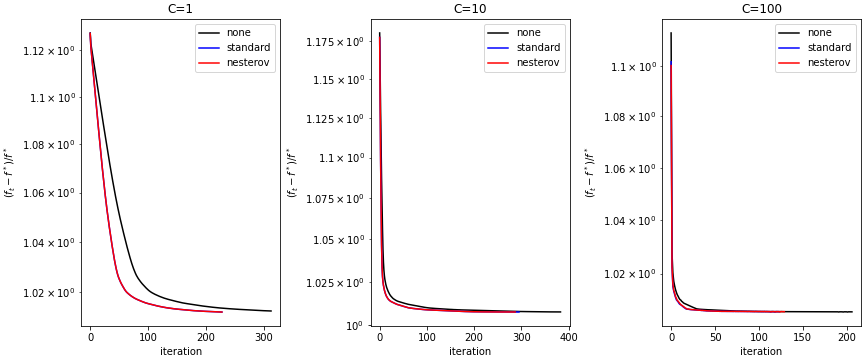
\includegraphics[scale=0.55]{img/l1_svc_loss_history}
	\caption{Loss convergence for the Primal formulation of the $\protect \mathcal{L}_1$-SVC}
	\label{fig:l1_svc_history}
\end{figure}

\paragraph{Linear Dual formulations}

The experiments results shown in~\ref{linear_lagrangian_dual_svc_cv_results} are obtained with $\alpha$, i.e., the \emph{learning rate} or \emph{step size}, setted to 0.001 for the \emph{AdaGrad} algorithm. Notice that the \emph{unreg\_bias} dual refers to the formulation~\eqref{eq:svc_lagrangian_dual}, while the \emph{reg\_bias} dual refers to the formulation~\eqref{eq:svc_bcqp_lagrangian_dual}.

\begin{table}[H]
\centering
\caption{Linear SVC Wolfe Dual formulation results with Hinge loss}
\label{linear_dual_svc_cv_results}
\begin{tabular}{llrrrr}
\toprule
       &     &  fit\_time &  accuracy &  n\_iter &  n\_sv \\
solver & C &           &           &         &       \\
\midrule
smo & 1   &  0.052323 &     0.980 &      62 &    17 \\
       & 10  &  0.091658 &     0.980 &     295 &    10 \\
       & 100 &  0.137948 &     0.985 &     399 &     8 \\
libsvm & 1   &  0.002719 &     0.985 &     243 &    17 \\
       & 10  &  0.002529 &     0.985 &     194 &    10 \\
       & 100 &  0.002797 &     0.985 &    1602 &     8 \\
cvxopt & 1   &  0.020693 &     0.980 &      10 &    17 \\
       & 10  &  0.023231 &     0.980 &      10 &    11 \\
       & 100 &  0.064602 &     0.985 &      10 &     8 \\
\bottomrule
\end{tabular}
\end{table}


For what about the linear \emph{Wolfe dual} formulation we can immediately notice as higher \emph{regularization hyperparameter} $C$ makes the model harder, so the \emph{custom} implementation of the SMO algorithm and also the \emph{sklearn} implementation, i.e., \emph{libsvm}~\cite{chang2011libsvm} implementation, needs to perform more iterations to achieve the same \emph{numerical precision}; meanwhile the \emph{cvxopt}~\cite{vandenberghe2010cvxopt} seems to be insensitive to the increasing complexity of the model. The results in terms of \emph{accuracy} and number of \emph{support vectors} are strongly similar to each others.

\begin{table}[H]
\centering
\caption{Linear SVC Lagrangian Dual formulation results with Hinge loss}
\label{linear_lagrangian_dual_svc_cv_results}
\begin{tabular}{llrrrr}
\toprule
     &     &  fit\_time &  accuracy &  n\_iter &  n\_sv \\
dual & C &           &           &         &       \\
\midrule
qp & 1   &  0.021188 &     0.985 &       1 &   195 \\
     & 10  &  0.007776 &     0.985 &       1 &   195 \\
     & 100 &  0.007696 &     0.985 &       1 &   195 \\
bcqp & 1   &  0.008790 &     0.985 &       1 &   194 \\
     & 10  &  0.008028 &     0.985 &       1 &   194 \\
     & 100 &  0.008192 &     0.985 &       1 &   194 \\
\bottomrule
\end{tabular}
\end{table}


For what about the linear \emph{Lagrangian dual} formulation we can see as it seems to be insensitive to the increasing complexity of the model in terms of number of \emph{iterations} but it tends to select many training data points as \emph{support vectors}.

\paragraph{Nonlinear Dual formulations}

The experiments results shown in~\ref{nonlinear_dual_svc_cv_results} and~\ref{nonlinear_lagrangian_dual_svc_cv_results} are obtained with \emph{d} and \emph{r} hyperparameters equal to 3 and 1 respectively for the \emph{polynomial} kernel; \emph{gamma} is setted to \emph{`scale`} for both \emph{polynomial} and \emph{gaussian RBF} kernels. The experiments results shown in~\ref{nonlinear_lagrangian_dual_svc_cv_results} are obtained with $\alpha$, i.e., the \emph{learning rate} or \emph{step size}, setted to 0.001 for the \emph{AdaGrad} algorithm.

\begin{table}[H]
\centering
\caption{Nonlinear SVC Wolfe Dual formulation results with Hinge loss}
\label{nonlinear_dual_svc_cv_results}
\begin{tabular}{lllrrrr}
\toprule
       &     &     &  fit\_time &  accuracy &  n\_iter &  n\_sv \\
solver & kernel & C &           &           &         &       \\
\midrule
smo & poly & 1   &  0.262513 &    0.6825 &     143 &    30 \\
       &     & 10  &  0.197470 &    0.9475 &      65 &    10 \\
       &     & 100 &  0.140720 &    0.9775 &      38 &     6 \\
       & rbf & 1   &  0.289481 &    1.0000 &      66 &    51 \\
       &     & 10  &  0.143812 &    1.0000 &      38 &    13 \\
       &     & 100 &  0.196509 &    1.0000 &      56 &    12 \\
libsvm & poly & 1   &  0.005542 &    1.0000 &     233 &    30 \\
       &     & 10  &  0.004144 &    1.0000 &     118 &    10 \\
       &     & 100 &  0.004042 &    1.0000 &      88 &     6 \\
       & rbf & 1   &  0.005162 &    1.0000 &     252 &    50 \\
       &     & 10  &  0.003994 &    1.0000 &     134 &    13 \\
       &     & 100 &  0.005558 &    1.0000 &     182 &    12 \\
cvxopt & poly & 1   &  0.208703 &    0.6775 &      10 &    31 \\
       &     & 10  &  0.194188 &    0.9475 &      10 &    10 \\
       &     & 100 &  0.228154 &    0.9775 &      10 &     6 \\
       & rbf & 1   &  0.177948 &    1.0000 &      10 &    50 \\
       &     & 10  &  0.239361 &    1.0000 &      10 &    19 \\
       &     & 100 &  0.206783 &    1.0000 &      10 &    17 \\
\bottomrule
\end{tabular}
\end{table}


\begin{table}[H]
\centering
\caption{Nonlinear SVC Lagrangian Dual formulation results with Hinge loss}
\label{nonlinear_lagrangian_dual_svc_cv_results}
\begin{tabular}{lllrrrr}
\toprule
     &     &     &  fit\_time &  accuracy &  n\_iter &  n\_sv \\
dual & kernel & C &           &           &         &       \\
\midrule
qp & poly & 1   &  0.160826 &     0.640 &       3 &   316 \\
     &     & 10  &  0.034587 &     0.640 &       3 &   316 \\
     &     & 100 &  0.053057 &     0.640 &       3 &   316 \\
     & rbf & 1   &  0.112672 &     0.860 &       9 &   307 \\
     &     & 10  &  0.144244 &     0.860 &       9 &   307 \\
     &     & 100 &  0.148839 &     0.860 &       9 &   307 \\
bcqp & poly & 1   &  1.139823 &     0.635 &     222 &   317 \\
     &     & 10  &  1.106476 &     0.635 &     222 &   317 \\
     &     & 100 &  1.317503 &     0.635 &     222 &   317 \\
     & rbf & 1   &  0.115288 &     1.000 &       1 &   399 \\
     &     & 10  &  0.057738 &     1.000 &       1 &   399 \\
     &     & 100 &  0.092722 &     1.000 &       1 &   399 \\
\bottomrule
\end{tabular}
\end{table}


The same considerations made for the previous linear \emph{Wolfe dual} and \emph{Lagrangian dual} formulations are confirmed also in the nonlinearly separable case. In this setting the complexity of the model coming with higher $C$ regularization values seems to be not paying a tradeoff in terms of the number of \emph{iterations} of the algorithm and, moreover, the \emph{reg\_bias Lagrangian dual} formulation seems to perform better wrt the \emph{unreg\_bias} formulation, both tends to select even more training data points as \emph{support vectors}.

\begin{figure}[H]
	\centering
	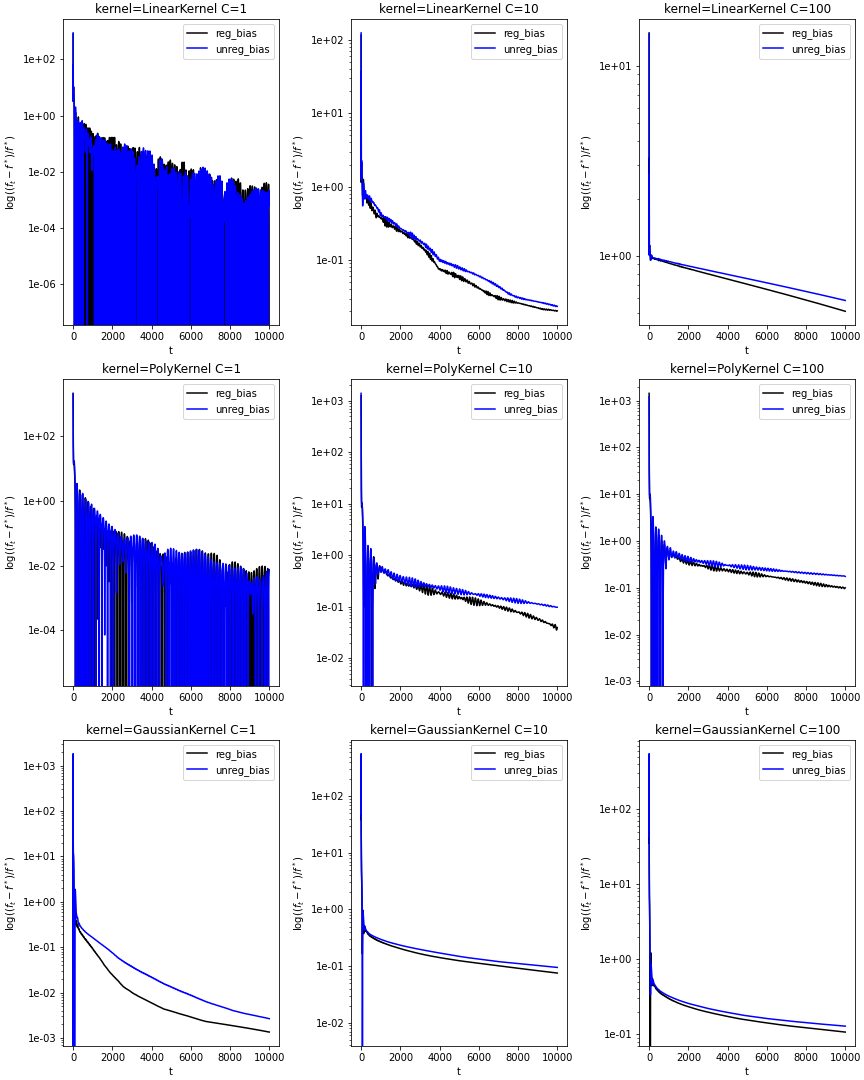
\includegraphics[scale=0.55]{img/lagrangian_dual_l1_svc_loss_history}
	\caption{Loss convergence for the Lagrangian Dual formulation of the Nonlinear $\protect \mathcal{L}_1$-SVC}
	\label{fig:lagrangian_dual_svc_loss_history}
\end{figure}

\pagebreak

\subsubsection{Squared Hinge loss}

\paragraph{Primal formulation}

The experiments results shown in~\ref{primal_l2_svc_cv_results} referred to \emph{Stochastic Gradient Descent} algorithm are obtained with $\alpha$, i.e., the \emph{learning rate} or \emph{step size}, setted to 0.001 and $\beta$, i.e., the \emph{momentum}, equal to 0.4. The batch size is setted to 20. Training is stopped if after 5 iterations the training loss is not lower than the best found so far.

\begin{table}[H]
\centering
\caption{SVC Primal formulation results with Squared Hinge loss}
\label{primal_l2_svc_cv_results}
\begin{tabular}{lllrrrr}
\toprule
          &   &     &  fit\_time &  accuracy &  n\_iter &  n\_sv \\
solver & momentum & C &           &           &         &       \\
\midrule
sgd & none & 1   &  0.419254 &     0.975 &     154 &    49 \\
          &   & 10  &  0.314466 &     0.980 &     119 &    24 \\
          &   & 100 &  0.079897 &     0.985 &      30 &    15 \\
          & standard & 1   &  0.312977 &     0.975 &     113 &    45 \\
          &   & 10  &  0.203847 &     0.980 &      73 &    24 \\
          &   & 100 &  0.061971 &     0.985 &      21 &    11 \\
          & nesterov & 1   &  0.328923 &     0.970 &     132 &    40 \\
          &   & 10  &  0.188573 &     0.980 &      71 &    23 \\
          &   & 100 &  0.073157 &     0.985 &      26 &    10 \\
liblinear & - & 1   &  0.002038 &     0.980 &     556 &    25 \\
          &   & 10  &  0.002624 &     0.980 &    1000 &    19 \\
          &   & 100 &  0.002467 &     0.980 &    1000 &    27 \\
\bottomrule
\end{tabular}
\end{table}


Again, the results provided from the \emph{custom} implementation, i.e., the SGD with different momentum settings, are strongly similar to those of \emph{sklearn} implementation, i.e., \emph{liblinear}~\cite{fan2008liblinear} implementation, in terms of \emph{accuracy} score. More training data points are selected as \emph{support vectors} from the SGD solver but it always requires even lower iterations, i.e., epochs, to achieve the same \emph{numerical precision}. \emph{Standard} or \emph{Polyak} and \emph{Nesterov} momentums always perform lower iterations as expected from the theoretical analysis of the convergence rate.

\begin{figure}[H]
	\centering
	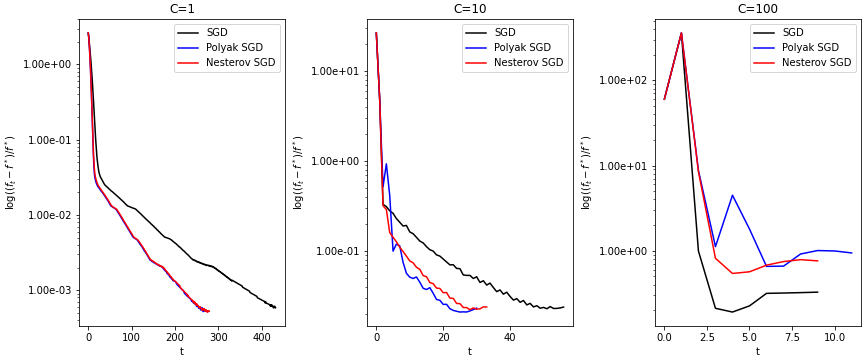
\includegraphics[scale=0.55]{img/l2_svc_loss_history}
	\caption{Loss convergence for the Primal formulation of the $\protect \mathcal{L}_2$-SVC}
	\label{fig:l2_svc_loss_history}
\end{figure}

\pagebreak

\subsection{Support Vector Regression}

Below experiments are about the SVR for which I tested different values for regularization hyperparameter $C$, i.e., from \emph{soft} to \emph{hard margin}, the $\epsilon$ penalty value and in case of nonlinearly separable data also different \emph{kernel functions} mentioned above.

\subsubsection{Epsilon-insensitive loss}

\paragraph{Primal formulation}

The experiments results shown in~\ref{primal_l1_svr_cv_results} referred to \emph{Stochastic Gradient Descent} algorithm are obtained with $\alpha$, i.e., the \emph{learning rate} or \emph{step size}, setted to 0.001 and $\beta$, i.e., the \emph{momentum}, equal to 0.4. The batch size is setted to 20. Training is stopped if after 5 iterations the training loss is not lower than the best found so far.

\begin{table}[H]
\centering
\caption{Primal $\protect \mathcal{L}_1$-SVR results}
\label{primal_l1_svr_cv_results}
\begin{tabular}{llllrrrr}
\toprule
          &   &     &     &   fit\_time &        r2 &  n\_iter &  n\_sv \\
solver & momentum & C & epsilon &            &           &         &       \\
\midrule
sgd & none & 1   & 0.1 &  13.207407 &  0.954298 &   16161 &   100 \\
          &   &     & 0.2 &   9.523358 &  0.954544 &   12267 &    99 \\
          &   &     & 0.3 &  11.594773 &  0.955424 &   13665 &    99 \\
          &   & 10  & 0.1 &   0.690761 &  0.983893 &     806 &    98 \\
          &   &     & 0.2 &   0.722907 &  0.983891 &     884 &    98 \\
          &   &     & 0.3 &   0.756686 &  0.983884 &     958 &    97 \\
          &   & 100 & 0.1 &   0.121053 &  0.984034 &      85 &    97 \\
          &   &     & 0.2 &   0.088140 &  0.984047 &      96 &    98 \\
          &   &     & 0.3 &   0.156799 &  0.984056 &     109 &    98 \\
          & polyak & 1   & 0.1 &   7.895537 &  0.954321 &    9874 &   100 \\
          &   &     & 0.2 &   5.816864 &  0.954549 &    7400 &    99 \\
          &   &     & 0.3 &   6.935173 &  0.955424 &    8200 &    99 \\
          &   & 10  & 0.1 &   0.489926 &  0.983893 &     487 &    97 \\
          &   &     & 0.2 &   0.503936 &  0.983891 &     535 &    98 \\
          &   &     & 0.3 &   0.483785 &  0.983885 &     569 &    98 \\
          &   & 100 & 0.1 &   0.090085 &  0.984030 &      48 &    98 \\
          &   &     & 0.2 &   0.108489 &  0.984046 &      56 &    98 \\
          &   &     & 0.3 &   0.114756 &  0.984055 &      61 &    97 \\
          & nesterov & 1   & 0.1 &   8.996545 &  0.954310 &    9785 &   100 \\
          &   &     & 0.2 &   6.001156 &  0.954546 &    7382 &    99 \\
          &   &     & 0.3 &   7.318327 &  0.955424 &    8198 &    99 \\
          &   & 10  & 0.1 &   0.803194 &  0.983892 &     489 &    97 \\
          &   &     & 0.2 &   0.457146 &  0.983890 &     533 &    97 \\
          &   &     & 0.3 &   0.561535 &  0.983884 &     579 &    98 \\
          &   & 100 & 0.1 &   0.097744 &  0.984031 &      61 &    98 \\
          &   &     & 0.2 &   0.120314 &  0.984047 &      58 &    98 \\
          &   &     & 0.3 &   0.107943 &  0.984057 &      62 &    98 \\
liblinear & - & 1   & 0.1 &   0.019717 &  0.954684 &      12 &   100 \\
          &   &     & 0.2 &   0.001534 &  0.955112 &      10 &    99 \\
          &   &     & 0.3 &   0.001302 &  0.955415 &      10 &    97 \\
          &   & 10  & 0.1 &   0.002194 &  0.983893 &      57 &    99 \\
          &   &     & 0.2 &   0.001483 &  0.983890 &      69 &    98 \\
          &   &     & 0.3 &   0.001968 &  0.983906 &     142 &    97 \\
          &   & 100 & 0.1 &   0.001972 &  0.984023 &     980 &    97 \\
          &   &     & 0.2 &   0.006431 &  0.984028 &    1340 &    97 \\
          &   &     & 0.3 &   0.002328 &  0.984051 &    2886 &    97 \\
\bottomrule
\end{tabular}
\end{table}


The results provided from the \emph{custom} implementation, i.e., the SGD with different momentum settings, are strongly similar to those of \emph{sklearn} implementation, i.e., \emph{liblinear}~\cite{fan2008liblinear} implementation, in terms of \emph{r2} score, except in case of $C$ regularization hyperparameter equals to 1 for which those of SGD are lower. Moreover, the SGD solver always requires lower iterations, i.e., epochs, for higher $C$ regularization values, i.e., for $C$ equals to 10 or 100, to achieve the same \emph{numerical precision}. Again, \emph{Standard} or \emph{Polyak} and \emph{Nesterov} momentums always perform lower iterations as expected from the theoretical analysis of the convergence rate. The results in terms of \emph{support vectors} are strongly similar to each others.

\begin{figure}[H]
	\centering
	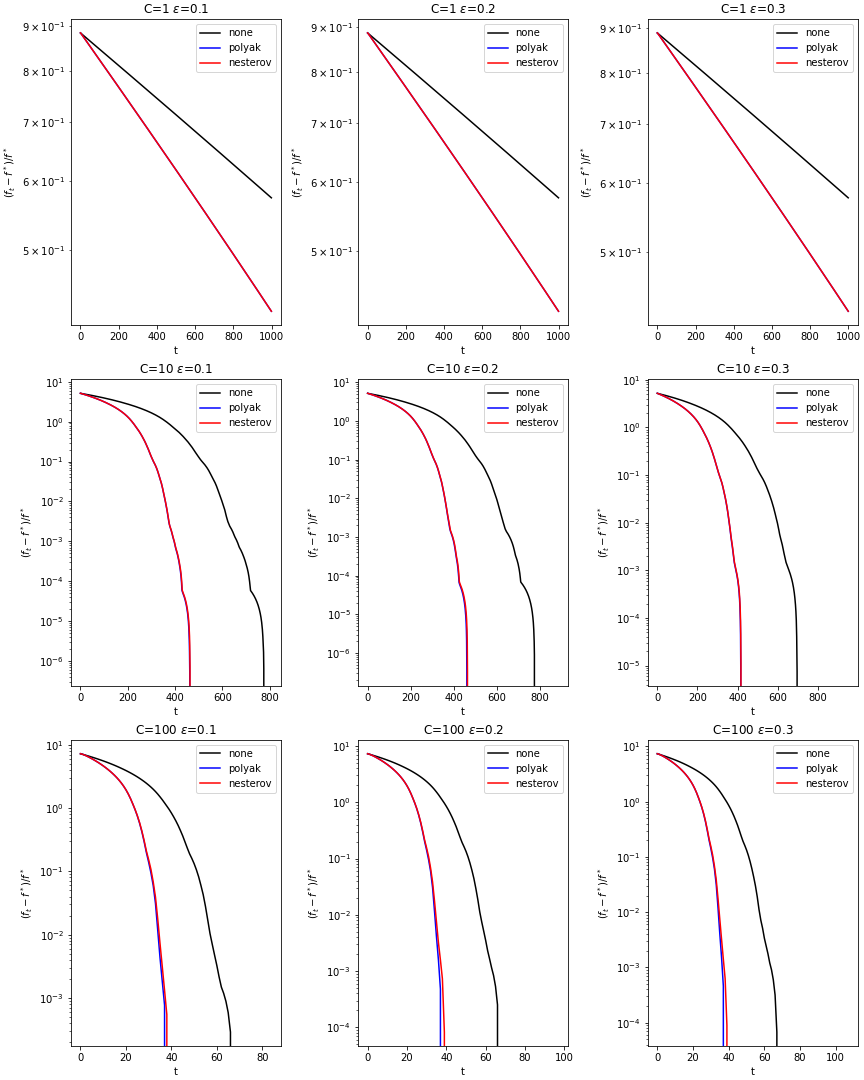
\includegraphics[scale=0.5]{img/l1_svr_loss_history}
	\caption{Loss convergence for the Primal formulation of the $\protect \mathcal{L}_1$-SVR}
	\label{fig:l1_svr_loss_history}
\end{figure}

\pagebreak

\paragraph{Linear Dual formulations}

The experiments results shown in~\ref{linear_lagrangian_dual_svr_cv_results} are obtained with $\alpha$, i.e., the \emph{learning rate} or \emph{step size}, setted to 0.001 for the \emph{AdaGrad} algorithm. Notice that the \emph{unreg\_bias} dual refers to the formulation~\eqref{eq:svr_lagrangian_dual}, while the \emph{reg\_bias} dual refers to the formulation~\eqref{eq:svr_bcqp_lagrangian_dual}.

\input{experiments/linear_dual_svr}

For what about the linear \emph{Wolfe dual} formulation we can immediately notice as higher \emph{regularization hyperparameter} $C$ and lower $\epsilon$ values makes the model harder, so the \emph{custom} implementation of the SMO algorithm and also the \emph{sklearn} implementation, i.e., \emph{libsvm}~\cite{chang2011libsvm} implementation, needs to perform more iterations to achieve the same \emph{numerical precision}; meanwhile, again, the \emph{cvxopt}~\cite{vandenberghe2010cvxopt} seems to be insensitive to the increasing complexity of the model. The results in terms of \emph{r2} and number of \emph{support vectors} are strongly similar to each others.

\begin{table}[H]
\centering
\caption{Linear SVR Lagrangian Dual formulation results with Epsilon-insensitive loss}
\label{linear_lagrangian_dual_svr_cv_results}
\begin{tabular}{lllrrrr}
\toprule
         &     &     &  fit\_time &        r2 &  n\_iter &  n\_sv \\
dual & C & epsilon &           &           &         &       \\
\midrule
unreg\_bias & 1   & 0.1 &  1.441291 &  0.733183 &    1000 &   100 \\
         &     & 0.2 &  1.340206 &  0.733183 &    1000 &   100 \\
         &     & 0.3 &  2.187842 &  0.733183 &    1000 &   100 \\
         & 10  & 0.1 &  1.959154 &  0.733183 &    1000 &   100 \\
         &     & 0.2 &  1.626009 &  0.733183 &    1000 &   100 \\
         &     & 0.3 &  1.702965 &  0.733183 &    1000 &   100 \\
         & 100 & 0.1 &  2.326519 &  0.733183 &    1000 &   100 \\
         &     & 0.2 &  1.761996 &  0.733183 &    1000 &   100 \\
         &     & 0.3 &  2.106777 &  0.733183 &    1000 &   100 \\
reg\_bias & 1   & 0.1 &  2.128727 &  0.731400 &    1000 &   100 \\
         &     & 0.2 &  1.345529 &  0.731400 &    1000 &   100 \\
         &     & 0.3 &  1.907465 &  0.731400 &    1000 &   100 \\
         & 10  & 0.1 &  1.447497 &  0.731400 &    1000 &   100 \\
         &     & 0.2 &  1.678308 &  0.731400 &    1000 &   100 \\
         &     & 0.3 &  1.620172 &  0.731400 &    1000 &   100 \\
         & 100 & 0.1 &  1.475333 &  0.731400 &    1000 &   100 \\
         &     & 0.2 &  3.142653 &  0.731400 &    1000 &   100 \\
         &     & 0.3 &  1.376226 &  0.731400 &    1000 &   100 \\
\bottomrule
\end{tabular}
\end{table}


For what about the linear \emph{Lagrangian dual} formulation we can see as it seems to be insensitive to the increasing complexity of the model in terms of number of \emph{iterations} and require many \emph{iterations} wrt the \emph{Wolfe dual} formulation.

\begin{figure}[H]
	\centering
	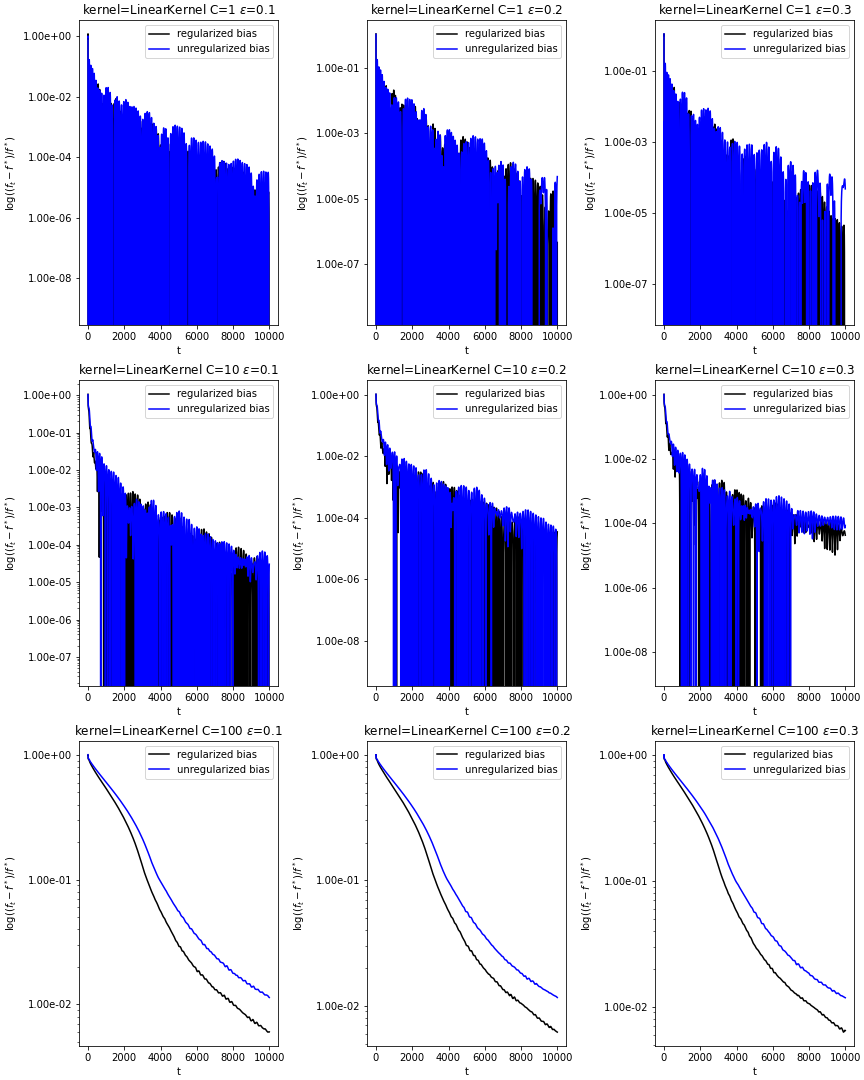
\includegraphics[scale=0.55]{img/linear_lagrangian_dual_l1_svr_loss_history}
	\caption{Loss convergence for the Lagrangian Dual formulation of the Linear $\protect \mathcal{L}_1$-SVR}
	\label{fig:lagrangian_dual_linear_svr_loss_history}
\end{figure}

\paragraph{Nonlinear Dual formulations}

The experiments results shown in~\ref{nonlinear_dual_svr_cv_results} and~\ref{nonlinear_lagrangian_dual_svr_cv_results} are obtained with \emph{d} and \emph{r} hyperparameters both equal to 3 for the \emph{polynomial} kernel; \emph{gamma} is setted to \emph{`scale`} for both \emph{polynomial} and \emph{gaussian RBF} kernels. The experiments results shown in~\ref{nonlinear_lagrangian_dual_svc_cv_results} are obtained with $\alpha$, i.e., the \emph{learning rate} or \emph{step size}, setted to 0.001 for the \emph{AdaGrad} algorithm.

\input{experiments/nonlinear_dual_svr}

\begin{table}[H]
\centering
\caption{Nonlinear SVR Lagrangian Dual formulation results with Epsilon-insensitive loss}
\label{nonlinear_lagrangian_dual_svr_cv_results}
\begin{tabular}{llllrrrr}
\toprule
     &     &     &     &  fit\_time &        r2 &  n\_iter &  n\_sv \\
dual & kernel & C & epsilon &           &           &         &       \\
\midrule
qp & poly & 1   & 0.1 &  1.426305 &  0.536892 &    1000 &   100 \\
     &     &     & 0.2 &  1.947305 &  0.536886 &    1000 &   100 \\
     &     &     & 0.3 &  1.597898 &  0.529220 &    1000 &   100 \\
     &     & 10  & 0.1 &  1.569864 &  0.536892 &    1000 &   100 \\
     &     &     & 0.2 &  1.659373 &  0.536886 &    1000 &   100 \\
     &     &     & 0.3 &  2.155713 &  0.529220 &    1000 &   100 \\
     &     & 100 & 0.1 &  2.127201 &  0.536892 &    1000 &   100 \\
     &     &     & 0.2 &  2.003470 &  0.536886 &    1000 &   100 \\
     &     &     & 0.3 &  1.385318 &  0.529220 &    1000 &   100 \\
     & rbf & 1   & 0.1 &  0.333465 &  0.733767 &     128 &   100 \\
     &     &     & 0.2 &  1.326574 &  0.718224 &     640 &   100 \\
     &     &     & 0.3 &  2.035441 &  0.580564 &    1000 &   100 \\
     &     & 10  & 0.1 &  0.369488 &  0.733767 &     128 &   100 \\
     &     &     & 0.2 &  1.663891 &  0.718224 &     640 &   100 \\
     &     &     & 0.3 &  1.971318 &  0.580564 &    1000 &   100 \\
     &     & 100 & 0.1 &  0.366429 &  0.733767 &     128 &   100 \\
     &     &     & 0.2 &  1.615145 &  0.718224 &     640 &   100 \\
     &     &     & 0.3 &  1.913055 &  0.580564 &    1000 &   100 \\
bcqp & poly & 1   & 0.1 &  1.363023 &  0.536344 &    1000 &   100 \\
     &     &     & 0.2 &  1.468118 &  0.536338 &    1000 &   100 \\
     &     &     & 0.3 &  1.414094 &  0.528759 &    1000 &   100 \\
     &     & 10  & 0.1 &  1.700776 &  0.536344 &    1000 &   100 \\
     &     &     & 0.2 &  1.394834 &  0.536338 &    1000 &   100 \\
     &     &     & 0.3 &  1.842973 &  0.528759 &    1000 &   100 \\
     &     & 100 & 0.1 &  2.344345 &  0.536344 &    1000 &   100 \\
     &     &     & 0.2 &  1.843466 &  0.536338 &    1000 &   100 \\
     &     &     & 0.3 &  1.377408 &  0.528759 &    1000 &   100 \\
     & rbf & 1   & 0.1 &  3.017241 &  0.739809 &    1000 &   100 \\
     &     &     & 0.2 &  0.320919 &  0.717846 &     165 &   100 \\
     &     &     & 0.3 &  0.398222 &  0.632389 &     185 &   100 \\
     &     & 10  & 0.1 &  2.460307 &  0.739809 &    1000 &   100 \\
     &     &     & 0.2 &  0.334468 &  0.717846 &     165 &   100 \\
     &     &     & 0.3 &  0.389869 &  0.632389 &     185 &   100 \\
     &     & 100 & 0.1 &  2.811035 &  0.739809 &    1000 &   100 \\
     &     &     & 0.2 &  0.336349 &  0.717846 &     165 &   100 \\
     &     &     & 0.3 &  0.400294 &  0.632389 &     185 &   100 \\
\bottomrule
\end{tabular}
\end{table}


The same considerations made for the previous linear \emph{Wolfe dual} and \emph{Lagrangian dual} formulations are confirmed also in the nonlinearly separable case. In this setting, the complexity of the model coming with higher $C$ regularization hyperparameters and lower $\epsilon$ values pays a larger tradeoff in terms of the number of \emph{iterations} of the algorithm.

\begin{figure}[H]
	\centering
	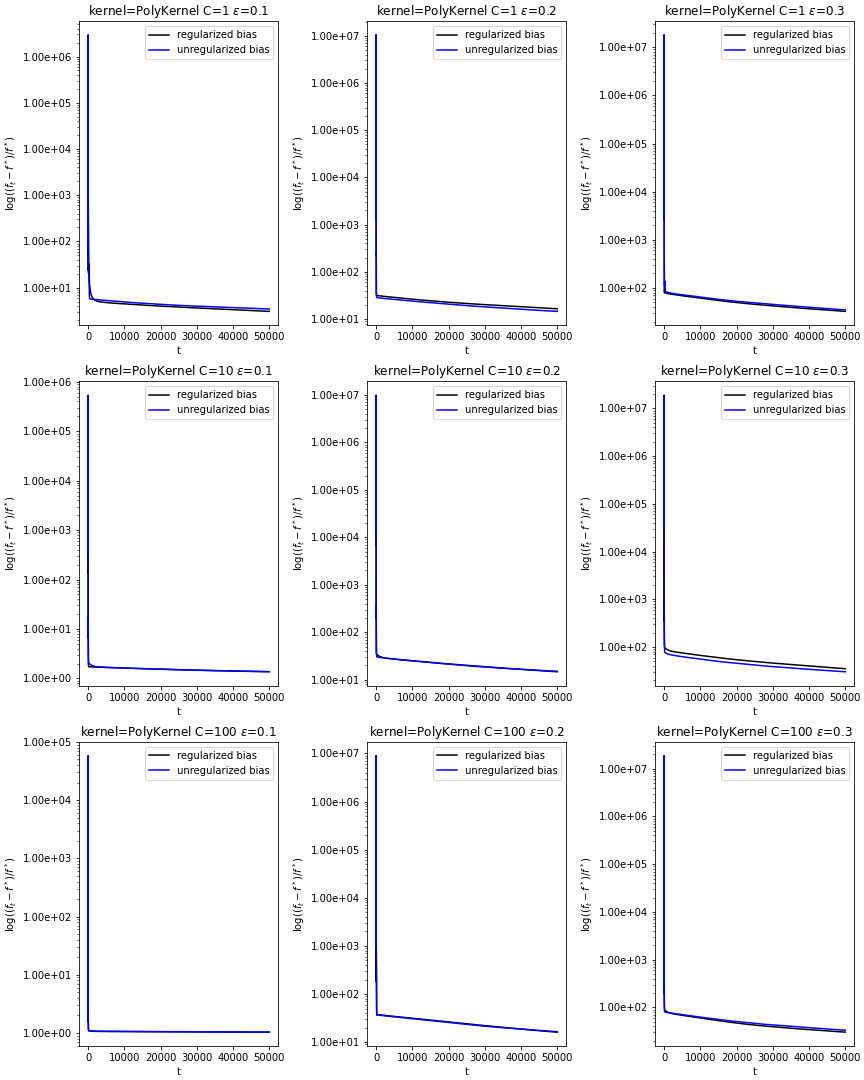
\includegraphics[scale=0.55]{img/poly_lagrangian_dual_l1_svr_loss_history}
	\caption{Loss convergence for the Lagrangian Dual formulation of the Polynomial $\protect \mathcal{L}_1$-SVR}
	\label{fig:lagrangian_dual_poly_svr_loss_history}
\end{figure}

\begin{figure}[H]
	\centering
	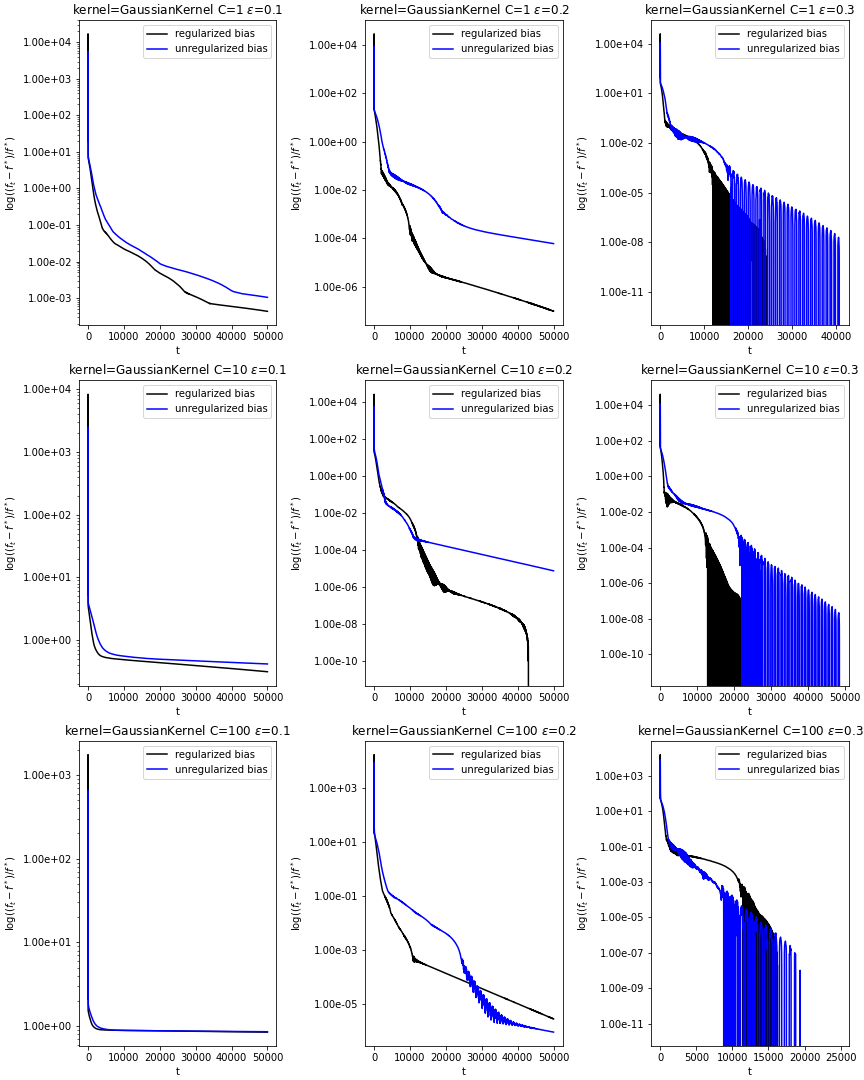
\includegraphics[scale=0.55]{img/gaussian_lagrangian_dual_l1_svr_loss_history}
	\caption{Loss convergence for the Lagrangian Dual formulation of the Gaussian $\protect \mathcal{L}_1$-SVR}
	\label{fig:lagrangian_dual_gaussian_svr_loss_history}
\end{figure}

\pagebreak

\subsubsection{Squared Epsilon-insensitive loss}

\paragraph{Primal formulation}

The experiments results shown in~\ref{primal_l2_svr_cv_results} referred to \emph{Stochastic Gradient Descent} algorithm are obtained with $\alpha$, i.e., the \emph{learning rate} or \emph{step size}, setted to 0.001 and $\beta$, i.e., the \emph{momentum}, equal to 0.4. The batch size is setted to 20. Training is stopped if after 5 iterations the training loss is not lower than the best found so far.

\begin{table}[H]
\centering
\caption{Primal $\protect \mathcal{L}_2$-SVR results}
\label{primal_l2_svr_cv_results}
\begin{tabular}{llllrrrr}
\toprule
          &   &     &     &  fit\_time &        r2 &  n\_iter &  n\_sv \\
solver & momentum & C & epsilon &           &           &         &       \\
\midrule
sgd & none & 1   & 0.1 &  0.628824 &  0.977019 &     652 &   100 \\
          &   &     & 0.2 &  0.604419 &  0.977008 &     655 &    99 \\
          &   &     & 0.3 &  0.594717 &  0.976996 &     657 &    99 \\
          &   & 10  & 0.1 &  0.069660 &  0.977572 &      75 &    99 \\
          &   &     & 0.2 &  0.069005 &  0.977572 &      75 &    99 \\
          &   &     & 0.3 &  0.070856 &  0.977571 &      76 &    99 \\
          &   & 100 & 0.1 &  0.008819 &  0.977413 &       8 &   100 \\
          &   &     & 0.2 &  0.009804 &  0.977418 &       9 &    99 \\
          &   &     & 0.3 &  0.009794 &  0.977423 &       9 &    98 \\
          & standard & 1   & 0.1 &  0.397914 &  0.977028 &     405 &   100 \\
          &   &     & 0.2 &  0.371360 &  0.977018 &     407 &    99 \\
          &   &     & 0.3 &  0.379346 &  0.977006 &     408 &    99 \\
          &   & 10  & 0.1 &  0.040419 &  0.977572 &      42 &    99 \\
          &   &     & 0.2 &  0.043567 &  0.977571 &      42 &    99 \\
          &   &     & 0.3 &  0.041749 &  0.977571 &      43 &    99 \\
          &   & 100 & 0.1 &  0.007162 &  0.977443 &       6 &    99 \\
          &   &     & 0.2 &  0.006814 &  0.977447 &       6 &    99 \\
          &   &     & 0.3 &  0.007255 &  0.977450 &       6 &    97 \\
          & nesterov & 1   & 0.1 &  0.403233 &  0.977028 &     406 &   100 \\
          &   &     & 0.2 &  0.376248 &  0.977018 &     408 &    99 \\
          &   &     & 0.3 &  0.379239 &  0.977006 &     409 &    99 \\
          &   & 10  & 0.1 &  0.040307 &  0.977572 &      43 &    99 \\
          &   &     & 0.2 &  0.043603 &  0.977571 &      43 &    99 \\
          &   &     & 0.3 &  0.041826 &  0.977570 &      43 &    99 \\
          &   & 100 & 0.1 &  0.007321 &  0.977417 &       6 &   100 \\
          &   &     & 0.2 &  0.007085 &  0.977423 &       6 &    99 \\
          &   &     & 0.3 &  0.007221 &  0.977428 &       6 &    98 \\
liblinear & - & 1   & 0.1 &  0.000905 &  0.977554 &      96 &   100 \\
          &   &     & 0.2 &  0.001104 &  0.977553 &      96 &   100 \\
          &   &     & 0.3 &  0.001333 &  0.977551 &      96 &   100 \\
          &   & 10  & 0.1 &  0.003077 &  0.977577 &     826 &   100 \\
          &   &     & 0.2 &  0.003161 &  0.977576 &     826 &    99 \\
          &   &     & 0.3 &  0.003165 &  0.977576 &     839 &    99 \\
          &   & 100 & 0.1 &  0.003899 &  0.977538 &    1000 &   100 \\
          &   &     & 0.2 &  0.003790 &  0.977540 &    1000 &    99 \\
          &   &     & 0.3 &  0.004260 &  0.977541 &    1000 &    98 \\
\bottomrule
\end{tabular}
\end{table}


Again, the results provided from the \emph{custom} implementation, i.e., the SGD with different momentum settings, are strongly similar to those of \emph{sklearn} implementation, i.e., \emph{liblinear}~\cite{fan2008liblinear} implementation, in terms of \emph{r2} score. SGD solver always requires even lower iterations, i.e., epochs, for higher $C$ regularization values, i.e., for $C$ equals to 10 or 100, to achieve the same \emph{numerical precision}. \emph{Standard} or \emph{Polyak} and \emph{Nesterov} momentums always perform lower iterations as expected from the theoretical analysis of the convergence rate.

\begin{figure}[H]
	\centering
	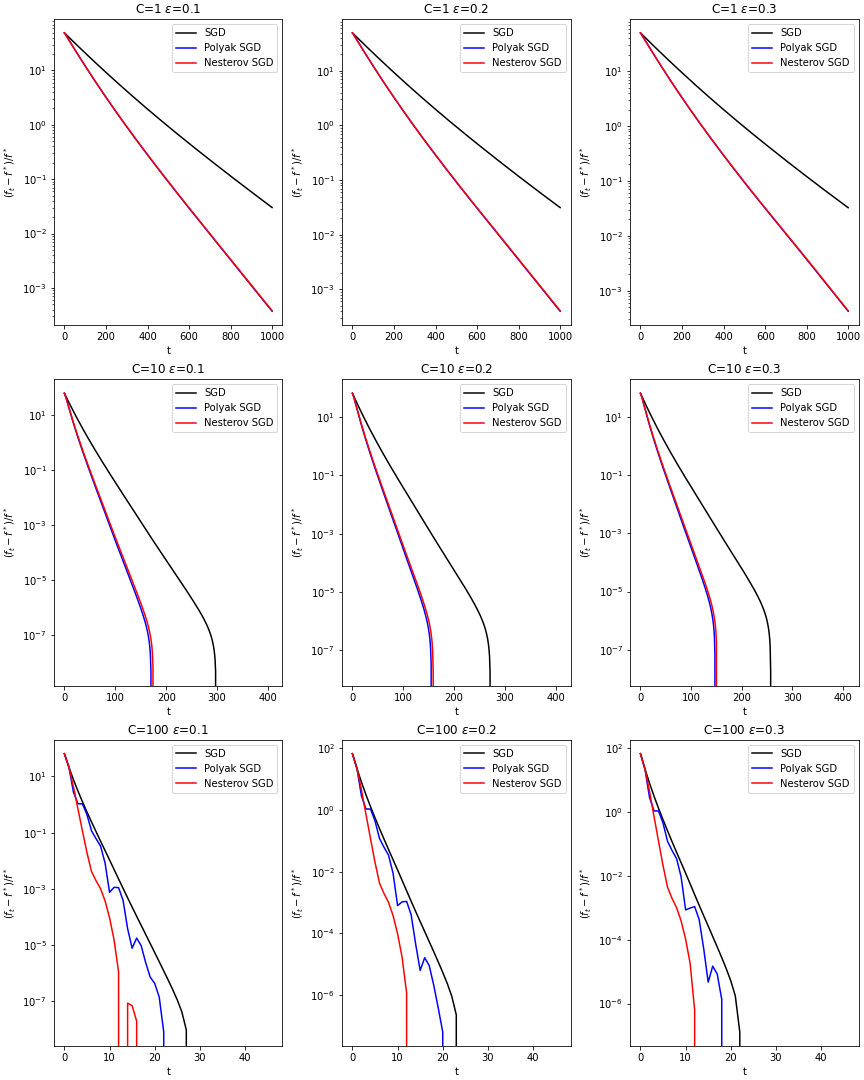
\includegraphics[scale=0.5]{img/l2_svr_loss_history}
	\caption{Loss convergence for the Primal formulation of the $\protect \mathcal{L}_2$-SVR}
	\label{fig:l2_svr_loss_history}
\end{figure}
